\documentclass[12pts]{report}

\usepackage[margin=1in]{geometry}
\usepackage[usenames, dvipsnames]{color}
\usepackage{setspace}
\usepackage{graphicx}
\doublespacing
\usepackage{fancyvrb}
\usepackage{varwidth}
\usepackage{verbatim}
\usepackage{multicol}
\usepackage{float}
\usepackage{fancyhdr}
\usepackage{parskip}    % This packages sets the spacing between two paragraphsc   
\usepackage{hyperref}              
\setlength{\parskip}{.5\baselineskip}   % Define spacing between two paragraphs

\setlength{\parindent}{0pt}
\setlength{\columnseprule}{0pt}

\pagestyle{fancy}
% Title Page
\title{DIME DYNAMIC DOCUMENTATION TRAINING \\ Exercise 2}
\author{Luiza Andrade \& Mrijan Rimal} 
\date{\today}

\fancyfoot{}
%\fancyhead[C]{\thepage}
\cfoot{\small{For the most recent version of the file, please check \url{https://github.com/worldbank/DIME-LaTeX-Templates/} } \\ \thepage}

\makeatother


\begin{document}
	
	
	\makeatletter
	\begin{titlepage}
		\begin{center}
			
\includegraphics[width=0.3\linewidth]{../img/i2i.png}\\[10ex]
			{\LARGE \bfseries  \@title }\\[2ex] 
			{\Large  \@author}\\[20ex] 
			{\large \@date}
		\end{center}
	\end{titlepage}
	\makeatother
	
\section*{Introduction}
Exercise 1 introduced you to the basics of how to import tables and figures to a {\LaTeX} document. This exercise will introduce you to some intermediate topics commonly used to make your document look even more professional.

We will also show how {\LaTeX} can be used to create a dynamic document that updates automatically once your output from, for example, Stata or R is updated without any error prone manual copy-and-pasting.

 

\section*{Exercise. Exporting tables}
Open \textcolor{red}{Export tables and images.do} and change the paths on the first section of the do-file so that it matches the folder structure you just created. Then run the do-file. This will export a few tables and graphs to the Raw folder that will be used in the following exercises.  \\

The following should be completed in this exercise: 
\begin{itemize}
	\item Make sure that you export \textbf{two tables} and \textbf{two graphs} using your own data. For help, you can look at the folder called ``Exercise Stata - How to export tables and graph from Stata to LaTeX''.
	\item Make sure that all the exporting is done using Stata do-files, or R scripts so you can easily export them again by just running the code. 
	\item Import all the tables and figures you have created in step 1 into your {\LaTeX} document using the templates provided in the \textbf{DIME Templates} sub-folder.
	\item Make sure you give a caption to your tables. 
\end{itemize}

\section*{Intermediate {\LaTeX} Exercises}
\subsection*{Adding Sections to your document}
{\LaTeX} automatically formats the document and different section headers and subheaders according to predefined formats. It also automatically creates beautiful \texttt{Table of Contents} based on what has been defined as sections and subsections. 

Sections can be created using \verb|\section{title}| command. {\LaTeX} automatically numbers all the sections in the order you put them. Since, you manually don't specify chapter numbers, you can cut and paste subsections from the end to the beginning and the numbering will update automatically! 

Similarly, subsections can be created using \verb|\subsection{title}| and sub-sub-sections can be created using \verb|\subsubsection{title}|. The subsections will be numbered 1.1 and the subsubsection will be number 1.1.1 if created within the first section. An example is shown in Annex 1\ref{sec:Annex}. 

\textit{Note: Sections and subsections can be created using} \verb|\section*{title}| \textit{if you do not want your sections numbered in the document. However, these sections and subsections will not be shown in the table of contents.}
\subsection*{Adding Table of Contents}

After we have set up sections, sub-sections and sub-sub-sections you can easily add a table of contents to your {\LaTeX} document by using \verb|\tableofcontents| in your docuemnt. You can create this any where you want, but typically this is created directly after \verb|\begin{document}| or after \verb|\maketitle| if you have a title.  An example is shown below:

\begin{multicols}{2}
	
\begin{Verbatim}[commandchars=+\(\)]
\documentclass[12pts]{article}

%opening
\title{My Awesome Document}
\author{John Doe}

\begin{document}
\maketitle
+color(CornflowerBlue)\tableofcontents
\newpage

\end{Verbatim}
The above {\LaTeX} code is used to generate table of contents.

\columnbreak
\begin{figure} [H]
	\centering
	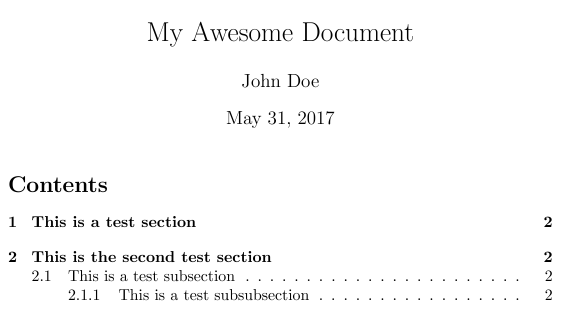
\includegraphics[width=1\linewidth]{../img/tableofcontents2}
	\caption{Example table of contents generated from our document in Annex 1.}
	\label{fig:tableofcontents}
\end{figure}
\end{multicols}

\subsection*{Referring to your tables, and figures in a document}

In this subsection, we will learn how to reference to a table, or a figure. 

To reference tables, or figures, we must give them a label to which we can refer to later. In Exercise 1, we learnt how to import a table/graph. We will now give the table and graph we imported in the previous exercise a label to make it easy to refer in the document. 

\subsubsection*{Referring to Figures in a document}
To add a label to the imported iegraph figure, we just add the lines \verb|\label{fig:Figurename}| inside the \texttt{begin} and \texttt{end} figure in our codes. 

\begin{Verbatim}[commandchars=+\(\)]
	\begin{figure}[H]
	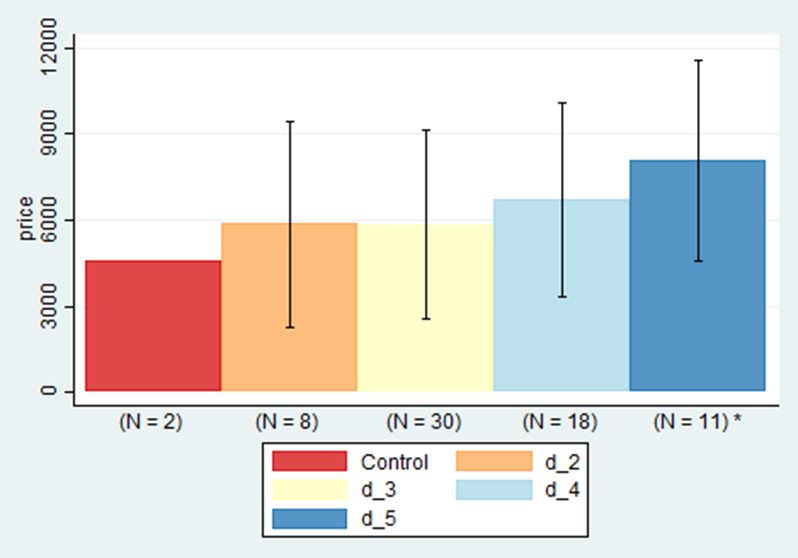
\includegraphics[width=\textwidth]{../Raw/iegraph.png}
	\caption{Add figure title here}
	+color(CornflowerBlue)\label{fig:iegraph}
	\end{figure}
\end{Verbatim}

Now to refer to the figure anywhere in the document, you can type \verb|\ref{fig:iegraph}| and it will automatically refer to the figure using the correct number in the document. In our example, if the \texttt{iegraph}	figure is the fourth one in the document, \verb|As you can see in figure \ref{fig:iegraph}| will appear as \texttt{As you can see in figure 4,} in the document. 

\subsubsection*{Referring to Tables in a document}

Similarly for tables, we can also refer to them anywhere in the document using the same method.

First, we need to add a label to the table that has been imported to the document by adding \verb|\label{tab:Tablename}| inside the \texttt{begin} and \texttt{end} table in our code. 

\begin{Verbatim}[commandchars=+\(\)]
\begin{table}[H]
\caption{Add a title to this table}
{
\def\sym#1{\ifmmode^{#1}\else\(^{#1}\)\fi}
\begin{tabular}{l*{4}{c}}
\hline\hline
          &\multicolumn{1}{c}{Group 1}&\multicolumn{1}{c}{Group 2}&\multicolumn{1}{c}{Group 3}&\multicolumn{1}{c}{Group 4}\\
\hline
Control   &       203         &       945         &        700         &        200         \\
Treatment &       151         &       952         &        952         &        148         \\
\hline
Total     &       354         &       1897         &       1652         &       348         \\
\hline\hline
\end{tabular}
}

+color(CornflowerBlue)\label{tab:samplesize}
\end{table}
\end{Verbatim}

Now we can refer to the above table in our document by typing \verb|\ref{tab:samplesize}| which will automatically refer to the table using the correct number in the document. 

\subsection*{Line Spacing}

Now that you have created sections in your document, and added text, you might want to change the spacing between lines. This can be achieved using the \texttt{setspace} package. 

The steps to change line spacing are as follows:
\begin{itemize}
	\item Before \verb|\begin{document}|, declare the package you will be using. In this case, \verb|\usepackage{setspace}|. This package controls the line spacing in a {\LaTeX} document.
	\item After using the \texttt{setspace} package, you should now specify line spacing which are as follows:
	\begin{description}
		\item[singlespacing] This option specifies the document to use one line spacing.
		\item[doublespacing] This option specifies the document to use two line spacing.
		\item[onehalfspacing] This option specifies the document to use one and a half line spacing. 
	\end{description}
\end{itemize}
\begin{Verbatim}[commandchars=+\(\)]
+color(CornflowerBlue)\usepackage{setspace}
+color(CornflowerBlue)\doublespacing
+color(Gray)%\onehalfspacing
+color(Gray)%\singlespacing
\begin{document}
\maketitle
\listoftables
\listoffigures
\section{Introduction}
This is the introduction paragraph
\end{Verbatim}
The \texttt{setspace} package can also be used to specify more particular linespacing i.e. 1.7 lines, 2.4 lines etc using the \texttt{setstretch} feature but that will be covered in another documents. 

\subsection*{Rotating a table landscape}

Sometimes the tables are very wide and need to be in landscape format. This can be adjusted using the \texttt{adjustbox} package which we have been using for importing tables. 

\begin{Verbatim}
\begin{table}[H]
	\caption{Add table title}
	{
\def\sym#1{\ifmmode^{#1}\else\(^{#1}\)\fi}
\begin{tabular}{l*{4}{c}}
\hline\hline
          &\multicolumn{1}{c}{Group 1}&\multicolumn{1}{c}{Group 2}&\multicolumn{1}{c}{Group 3}&\multicolumn{1}{c}{Group 4}\\
\hline
Control   &       203         &       945         &        700         &        200         \\
Treatment &       151         &       952         &        952         &        148         \\
\hline
Total     &       354         &       1897         &       1652         &       348         \\
\hline\hline
\end{tabular}
}

	\label{tab:samplesize}
\end{table}
\end{Verbatim}
To rotate the table to landscape, we can use the \texttt{adjustbox} feature with the \texttt{angle = 90} option as shown in blue in the code below.
\begin{Verbatim}[commandchars=+\(\)]
\begin{table}[H]
	\caption{Add table title}
+color(CornflowerBlue)	\begin{adjustbox}{angle = 90} 
		{
\def\sym#1{\ifmmode^{#1}\else\(^{#1}\)\fi}
\begin{tabular}{l*{4}{c}}
\hline\hline
          &\multicolumn{1}{c}{Group 1}&\multicolumn{1}{c}{Group 2}&\multicolumn{1}{c}{Group 3}&\multicolumn{1}{c}{Group 4}\\
\hline
Control   &       203         &       945         &        700         &        200         \\
Treatment &       151         &       952         &        952         &        148         \\
\hline
Total     &       354         &       1897         &       1652         &       348         \\
\hline\hline
\end{tabular}
}

+color(CornflowerBlue)	\end{adjustbox}
\label{tab:samplesize}
\end{table}
\end{Verbatim}

This will rotate the table to the specified degree in the final document. 

\section*{Making a Dynamic Document}

Here, we will produce a dynamic document. Please only do this do \textbf{if} you have completed up to \texttt{Part 5, Task 2} of the exercise. 

\begin{enumerate}
	\item Save the pdf created up to now in a separate location from your \texttt{.tex} file. 
	\item Generate a new treatment for your dataset by dropping some observations, using a different metric to create treatments, etc. 
	\item Rerun the do-file with the new treatment. Make sure that the tables and graphs you created earlier are overwritten. 
	\item Now, open the earlier created {\LaTeX} file and press \textit{Build and Compile} under the \textit{Tools}.
	\item Now if you compare the pdf file you have just generated with the one you saved earlier, you will find that the tables would have updated automatically. 
\end{enumerate}

\section*{Challenge: Using a do-file to edit a .tex file after exporting it}
\textit{Note: This is an advanced exercise and you don't have to feel compelled to finish it. This is also best done after finishing all the other exercises in the GitHub repository.}
 
During this part of the exercise, you will learn how to use commands in Stata to format your tables. While tables exported from Stata to {\LaTeX} are generally very nice, sometimes they need to be tweaked a little to make them look nicer. So, in this exercise, you'll use the \texttt{filefilter} command in Stata to make small changes to the files exported by Stata. 

This exercise requires more familiarity with {\LaTeX} than the previous. Don't worry if you can't complete it. 

\begin{description}
	\item[Task 1:] Run the initial code for exercise 6 in the \textcolor{red}{Add path and name of do-file} do-file. This will create a table with sample sizes for control and treatment groups across regions and in the whole sample. Add this table to the .tex file you created in the previous exercises. How does that look?
	\item[Task 2:] Open the \textcolor{red}{Add path and name of tex file} .tex file created by Stata. Can you identify the source of the extra spacing?
	\item[Task 3:] Use the \texttt{filefilter} command in Stata to filter out the lines or characters in the fragmented file that create the extra spacing. Import the new .tex file and check how it looks.
	\item[Task 4:] Repeat task 3 if necessary.
\end{description}


\newpage
\section*{Annex 1 : Creating sections}
\label{sec:Annex}
\begin{figure}[H]
	\centering
	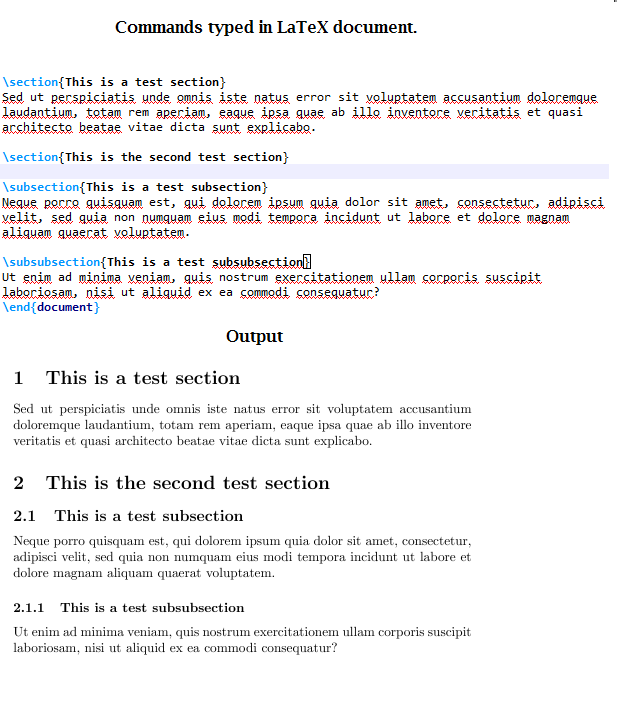
\includegraphics[width=0.7\linewidth]{../img/section}
	\caption{Adding sections and subsections in a {\LaTeX} document}
	\label{fig:adding sections}
\end{figure}
\end{document}          
